\documentclass{beamer}
%[aspectratio=169]   \usepackage[czech]{babel}
\usepackage{apo-lecture-en}
\usepackage{pdfpages}
\usepackage{pdfcomment}
\usepackage{listings}
\usepackage{array,multirow}

\subtitle{Lecture 07. Input and Output}
\author{Pavel Píša \phantom{xxxxxxxxx} Petr Štěpán \\ \small\texttt{pisa@fel.cvut.cz}\phantom{xxxx}\small\texttt{stepan@fel.cvut.cz}}
\begin{document}

\maketitle

\section{Input and Output}

\begin{frame}
\frametitle{Today's Lecture Objective}

\begin{itemize}
 \item Review what are the input and output options in a computer
 \item Memory-mapped peripherals
 \item Examples in QtRvSim
 \item PCI and PCIe buses
\end{itemize}
\end{frame}

\begin{frame}[shrink=10]
\frametitle{Computer Architecture -- John von Neumann}
\begin{center}
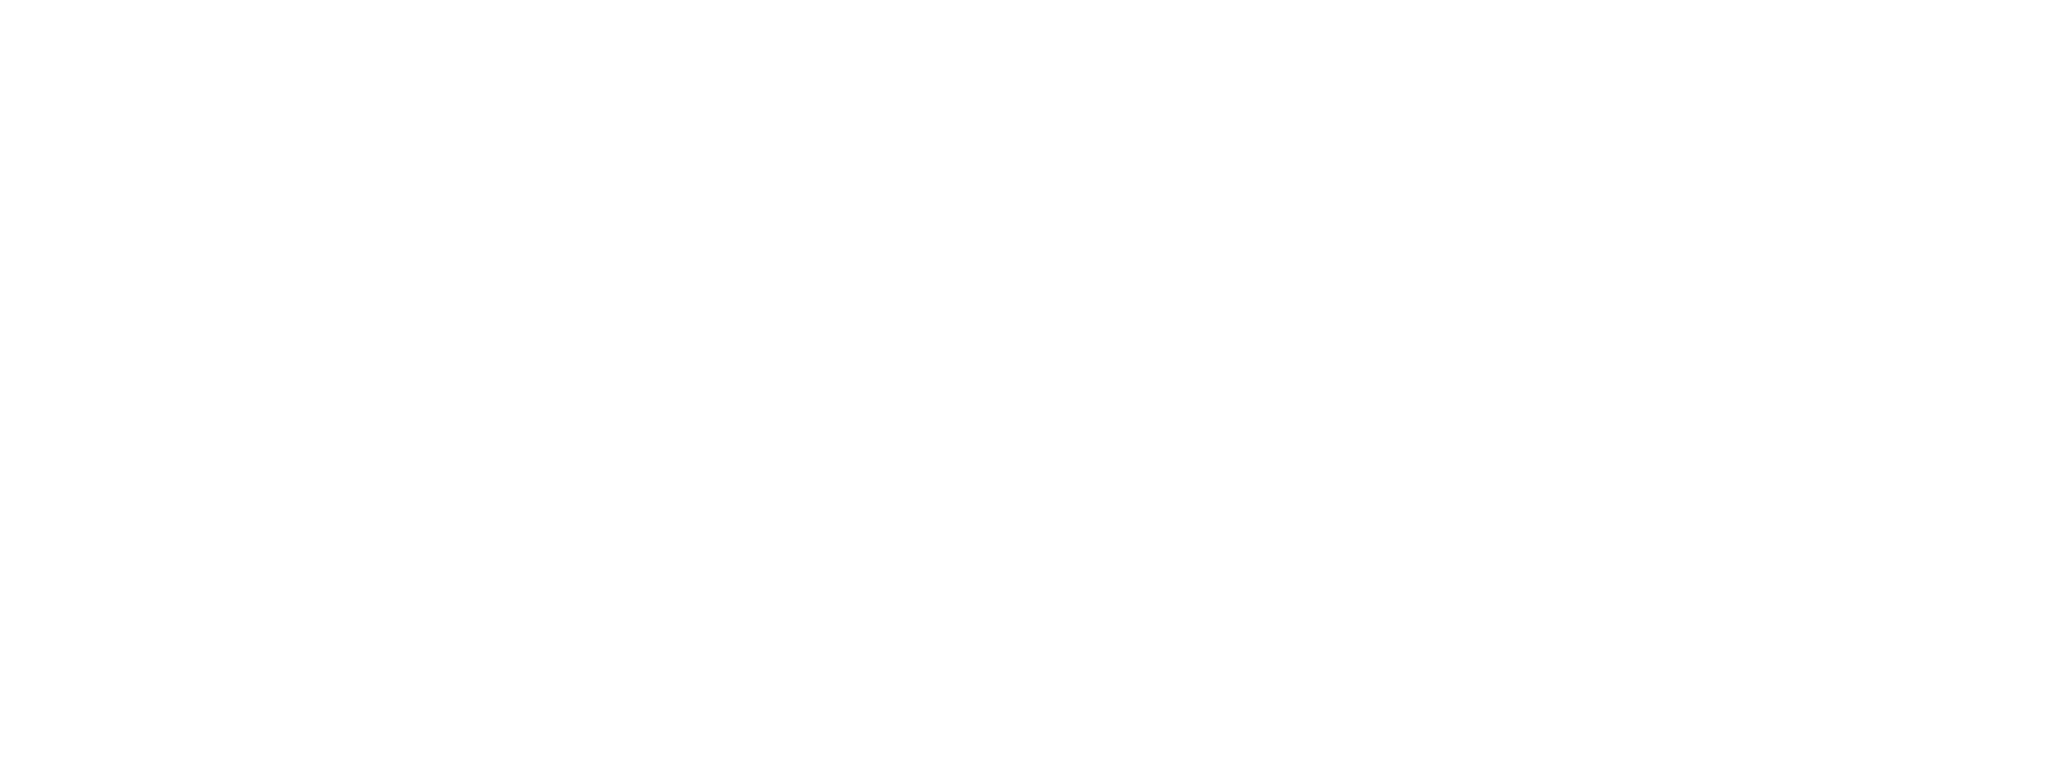
\includegraphics[width=0.5\textwidth]{cpu-vonNeumann.pdf}
\hfill
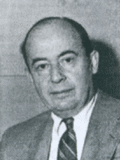
\includegraphics[width=0.15\textwidth]{fig/vonNeumann.png}
\end{center}
\begin{itemize}
\item 5 basic units – control unit, arithmetic-logic unit, memory, input (input device), output (output device)
\item The architecture of a computer should not depend on the task being solved, it should be able to execute a program stored in memory. The program controls which sequence of instructions computer executes and thus what results are computed.
\item The program and data are stored in the same memory, composed of cells (units) of the same size. In contrast, the Harvard architecture had one type of memory for the program and another type of memory for data.
\item The next instruction to be executed is stored in the next memory location (excluding program jumps)
\item Instructions perform arithmetic and logical operations, data transfers to/from memory, program jumps and branches, and special control instructions.
\end{itemize}
\end{frame}


\begin{frame}
\frametitle{Classification of Input/Output Devices/Peripherals}
By behavior:
\begin{itemize}
\item Input (read only)
\item Output (write only, cannot be read)
\item Input and output (currently, most devices, including keyboards -- they have an LED output)
\end{itemize}

By connection:
\begin{itemize}
\item Direct connection between CPU and peripherals
\item Hierarchical -- connection via other peripherals (bridge, switch)
\end{itemize}

By partner kind:
\begin{itemize}
\item Human -- other communication parameters
\item Computer -- usually faster communication
\item Environment -- sensors and actuators
\end{itemize}

By communication link/bus parameters:
\begin{itemize}
\item Capacity/badwidth of the link -- maximum data transfer capabilities
\item Latency -- time in which data transfer is performed
\end{itemize}
\end{frame}

\begin{frame}
\frametitle{Classification Peripherals -- Continues}

Examples of human-machine peripherals:
\begin{itemize}
\item keyboard -- only input, but often output on LED diodes, very small transmission speed, latency up to 200ms (except games playing)
\item  microphone/speakers -- transfer speed up to 8Mb/s, latency depends on application, for interactive communication (i.e. calls) requires latency of less than 500 ms, optimally 150 -- 300 ms
\item printer/scanner -- transfer speed according to connection, latency does not matter (in seconds / minutes)
\end{itemize}

Examples of peripherals for communication between computers
\begin{itemize}
\item modem -- modems 115.2\,kb/s (the first 200 b/s), LTE max 300\,Mb/s, 5G to 500\,Mb/s
\item network/WLAN -- from 10\,Mb/s to 1\,Gb/s to 1\,Tb/s
\item data storage -- HDD, SSD, magneto-tape units, communication speed according to connection (later today), SSD latency best, HDD worse, magneto-tape units -- only sequential writing possible
\end{itemize}

\end{frame}


\begin{frame}
\frametitle{Classification Peripherals -- Continues}

Examples of sensors and actuators:
\begin{itemize}
\item cameras, laser rage finders -- communication speed by type of connection
\begin{itemize}
\item USB 2.0 max 480\,Mb/s,
\item USB 3.1 max 5\,Gb/s,
\item WLAN up to 10\,Gb/s
\end{itemize}
\item actuators -- DC/PMSM motors
\begin{itemize}
\item transfer speed not so important, but latency
\item latency is the most important parameter for control
\item DC -- latency 0.5--0.05\,ms,
\item PMSM -- latency 0.05--0.01\,ms
\end{itemize}
\end{itemize}

\end{frame}


\begin{frame}
\frametitle{CPU Design from Lecture 5}
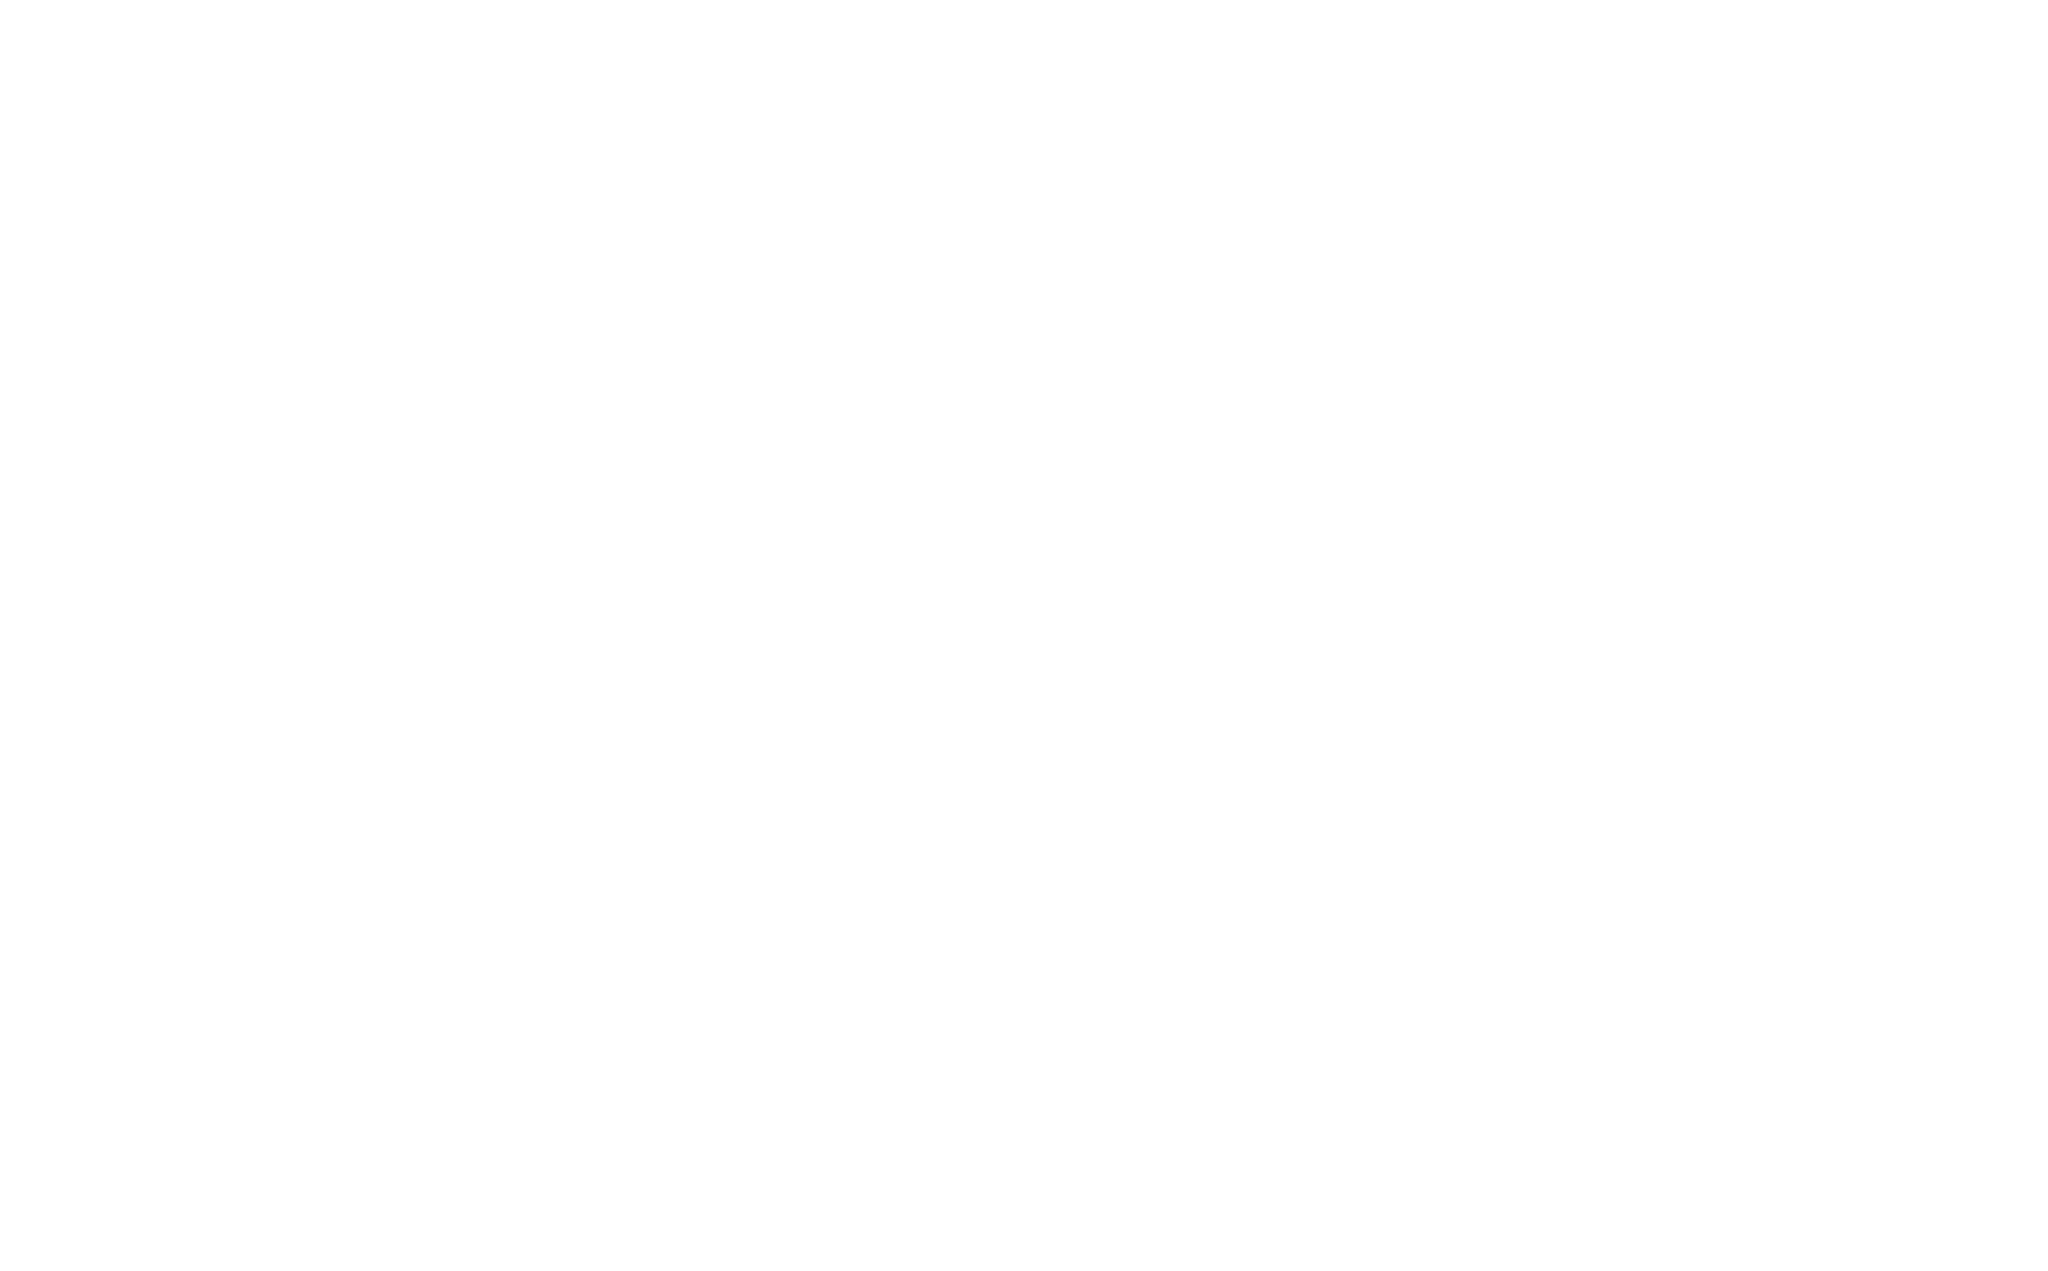
\includegraphics[width=0.95\textwidth]{cpu_design2.pdf}
\end{frame}


\begin{frame}
\frametitle{CPU Connection with Memory and Peripherals}
\begin{columns}
\begin{column}{0.4\textwidth}
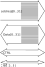
\includegraphics[width=0.9\textwidth]{bus_arch-en.pdf}
\end{column}
\begin{column}{0.6\textwidth}
\begin{itemize}
\item The address bus (A0..A31) can be separated or multiplexed, or share the same signals as the data part
\item Data bus (D0.. D31) can be bidirectional or separated for each direction, parallel or serial
\begin{itemize}
\item Example in the picture -- parallel 32-bit bus, the half-duplex data path using same signals for both directions
\end{itemize}
\item Control bus signals
\begin{itemize}
\item It controls the communication on the bus, direction, when transfer starts, ends, if the delay is required
\end{itemize}
\item BE0 to 3 -- controls write (even read sometimes) of individual bytes on a bus wider than 8 bits.
\end{itemize}
\end{column}
\end{columns}
\end{frame}


\begin{frame}
\frametitle{CPU Peripherals Access}

Two different approaches used:
\begin{itemize}
\item Special instructions for input/output
\begin{itemize}
\item "x86" uses the instructions \texttt{in}, \texttt{out}.
\item These instructions are similar to memory access ones, but data are read and written on the bus where peripherals are connected and or with special control signals.
\item The modern peripherals need often block access and larger addressing ranges for which memory access oriented instructions serve better and separated signalling for I/O access only complicates hardware and CPU.
\end{itemize}
\item Part of common (memory) address space reserved for input/output
\begin{itemize}
\item The RISC (including RISC-V) and even lot of CISC CPUs do not have special instructions for communication with peripherals, and therefore use same method and instructions as are used for reading and writing into data memory.
\item This methods is often runtime configurable, the peripherals are mapped into reserved address range that serves to move data between CPU and peripherals.
\end{itemize}
\end{itemize}
\end{frame}


\begin{frame}
\frametitle{Memory Mapped Peripherals -- RISC-V}

\begin{itemize}
\item There are no special instructions to access peripherals on RISC-V \item The same instruction are used for peripheral access as for load and store into data memory.
\item Address Decoder -- controls where are data sent/which device is read
\end{itemize}
\begin{center}
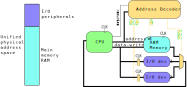
\includegraphics[width=0.88\textwidth]{address_decoder-en.pdf}
\end{center}
\end{frame}


\begin{frame}
\frametitle{Address Decoders Realizations}

Central decoder (one per system or bus)

\begin{center}
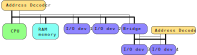
\includegraphics[width=0.8\textwidth]{central-en.pdf}
\end{center}

Autonomous -- peripheral local/decentralized decoders

\begin{center}
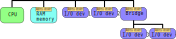
\includegraphics[width=0.8\textwidth]{distributed-en.pdf}
\end{center}
\end{frame}



\begin{frame}
\frametitle{Options to Exchange Data and Wait for Peripheral}
Software active (busy) polling:
\begin{itemize}
\item The device waits for CPU access and sends data to output, or provides already received input
\item If the data sending or availability is slower than CPU then CPU has to poll/read device status register (bits data ready/space available)
\end{itemize}

Interrupt driven/timed access to peripheral:
\begin{itemize}
\item If the state changes (data became ready, space is available) hardware signals interrupt (lecture 9)
\item This activates interrupt service handler and CPU then reads or writes data under SW control
\end{itemize}

Peripheral uses direct memory access:
\begin{itemize}
\item Uses interrupt for availability signalling as well
\item The CPU sets only from/to which address in the memory data will be read/written and the periphery itself controls data transfer
\item Peripheral signals by interrupt that all data/packet is ready to be processed by CPU or next one should be prepared by CPU
\end{itemize}

\end{frame}

\begin{frame}
\frametitle{Input/Output and Drivers in Linux Kernel (simplified)}
\begin{columns}
\begin{column}{0.4\textwidth}
The programs communicate with the peripherals using the operating system and system call and periphery drivers (overview in lecture 10, detailed in the OSY course -- Operating Systems).
\bigskip

Another option is direct access from the user application by mapping peripheral into process space -- the next topics of today's lecture. Low level kernel driver works similar way.
\end{column}
\begin{column}{0.58\textwidth}
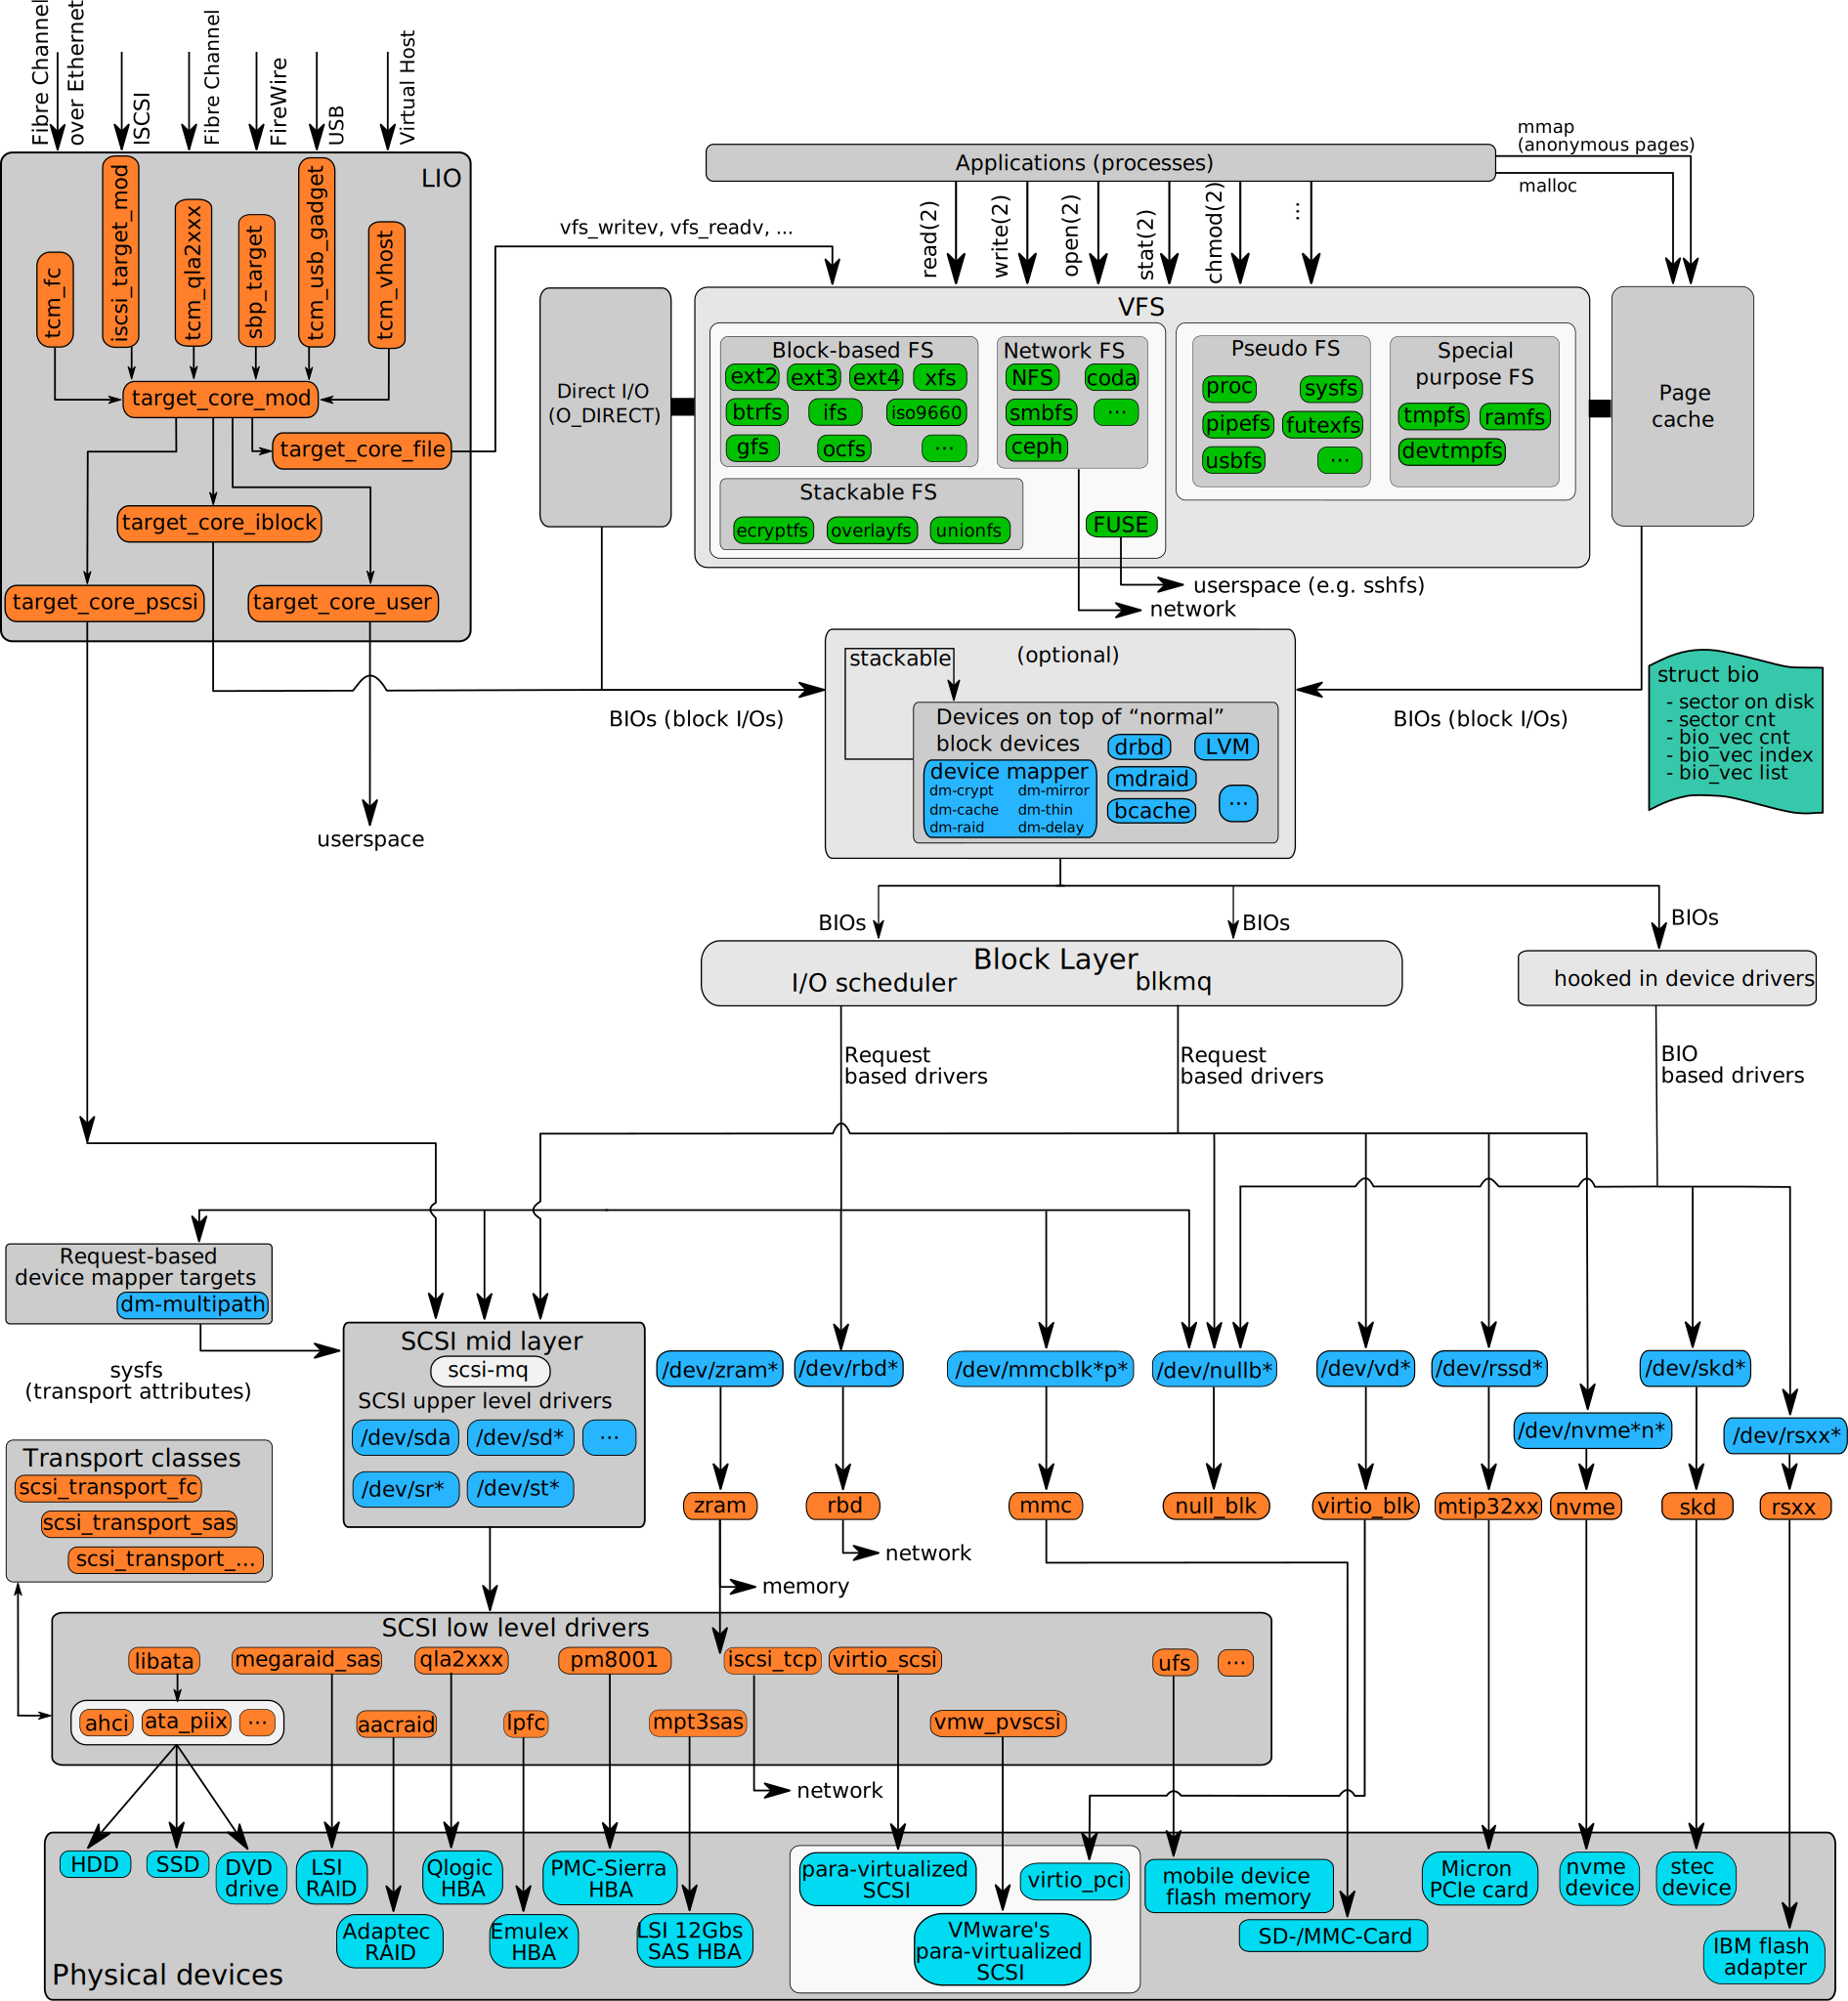
\includegraphics[width=\textwidth]{linux.pdf}
\end{column}
\end{columns}
\end{frame}


\begin{frame}
\frametitle{System Calls and Services}

System calls:
\begin{itemize}
\item system calls are wrapped as regular C functions in libc library functions and offered to user applications -- POSIX API
\item open function/system call
    \begin{itemize}
    \item for each periphery can be created handle same as for file
    \item this "file" handle is used to communicate with the peripheral
    \end{itemize}
\item read function/system call
    \begin{itemize}
    \item reads the data from the periphery same as data are read from the file
    \item blocking operation
        \begin{itemize}
        \item if no data are available, the function waits for at least one byte or packed arrival
        \item the process execution is suspended by operating system and does not block CPU
        \end{itemize}
    \item non-blocking operation
        \begin{itemize}
        \item if no byte/char is available, function return -1 and errrno EAGAIN/EWOULDBLOCK
        \item the process is responsible for waiting (i.e. by poll or select calls)
        \item received data are stored into internal buffers by the driver up to allocated buffers capacity
        \end{itemize}
    \end{itemize}
\end{itemize}
\end{frame}





\begin{frame}
\frametitle{Quiz}

the scanf function (read formatted input) behavior if data are not currently available to fill/parse into all specified fields:

\begin{itemize}
\item[A] actively repeats call to check wheather data are available
\item[B] the process is suspended and it is necessary to restart it
\item[C] the process is suspended and it is woken u by operating system when data arrives
\item[D] the function returns -1
\end{itemize}
\end{frame}



\section{QtRvSim Peripherals}

\begin{frame}
\frametitle{QtRvSim -- Rotary Knobs and RGB LEDs}

\begin{itemize}
\item the same data format for RGB LEDs as for reads of the rotary knobs state
\begin{itemize}
\item only bits 24 -- 31 are not used for RGB LEDs
\end{itemize}
\end{itemize}

\begin{table}
\scriptsize
\begin{tabular}{|m{1.0cm}|m{1.1cm}|m{0.5cm}|m{0.5cm}|m{0.5cm}|m{1.1cm}|m{1.1cm}|m{1.1cm}|}\hline
Bits & 31 ... 27 & 26 & 25 & 24 & 23 ... 16 & 15 ... 8 & 7 ... 0 \\ \hline
Meaning & not used & red push. & green push. & blue push. & red value & green value & blue value \\ \hline
\end{tabular}
\end{table}


\begin{itemize}
\item one word sized register on appropriate address for each RGB LED color value store, all three knobs state is read from the single 32-bit word size register/address
\item the write of the value to RGB LED register changes its color and intensity to written value immediately
\item the read of the register at rotary knobs representing address returns state of the knobs at the current time
\end{itemize}

\end{frame}


\begin{frame}[fragile]
\frametitle{QtRvSim -- Rotary Knobs and RGB LEDs}

\begin{columns}
\begin{column}{0.6\textwidth}
\begin{minted}[fontsize=\footnotesize]{gas}
# base of SPILED port region
.equ SPILED_REG_BASE,       0xffffc100

# RGB LED 1 - color components, 8 bits each
.equ SPILED_REG_LED_RGB1,   0xffffc110
.equ SPILED_REG_LED_RGB1_o,   0x0010

# RGB LED 2 - color components, 8 bits each
.equ SPILED_REG_LED_RGB2,   0xffffc114
.equ SPILED_REG_LED_RGB2_o,   0x0014

# read 8-bit color component value for each
# knob and knob push states in the MSB
.equ SPILED_REG_KNOBS_8BIT, 0xffffc124
.equ SPILED_REG_KNOBS_8BIT_o, 0x0024

# 32 LEDs - each of 32 bits controls one LED
.equ SPILED_REG_LED_LINE,   0xffffc104
.equ SPILED_REG_LED_LINE_o,   0x0004
\end{minted}
\end{column}
\begin{column}{0.4\textwidth}
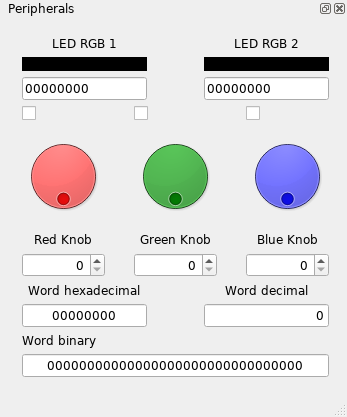
\includegraphics[width=\textwidth]{fig/knobs.png}
\end{column}
\end{columns}

\end{frame}

\begin{frame}[fragile]
\frametitle{Example of Using Rotary Knobs Value to Control RGB}

\begin{minted}[fontsize=\footnotesize]{gas}
    # a0 set to provide base for SPILED I/O memory mapped region
    li   a0, SPILED_REG_BASE
    ori  t2, t2, -1
loop:
    # read values from rotary knobs
    lw   t0, SPILED_REG_KNOBS_8BIT_o(a0)
    # set RGB LED 1 to corresponding color
    sw   t0, SPILED_REG_LED_RGB1_o(a0)
    xor  t1, t0, t2
    # set RGB LED 2 to complementary color
    sw   t1, SPILED_REG_LED_RGB2_o(a0)
    srli t0, t0, 24
    andi t0, t0, 4
    beq  t0, zero, loop       # repeat until red knob is pressed

    ebreak                    # stop/finish the program
\end{minted}
\end{frame}

\begin{frame}
\frametitle{Quiz -- Rotary Knobs}

Choose how to obtain value of the green knob if the 32-bit/word value representing position of the knobs is read from \texttt{SPILED\_REG\_BASE+SPILED\_REG\_KNOBS\_8BIT\_o} register  and stored into variable \texttt{unsigned int v;}. Available solutions:
\begin{itemize}
\item[A] \texttt{((v<<24) \& 0x00ff00)}
\item[B] \texttt{((v>>8) \& 0xff)}
\item[C] \texttt{(v \& 0x30303030)}
\item[D] \texttt{((v>>24) \& 0xf0)}
\end{itemize}
\end{frame}



\begin{frame}
\frametitle{Asynchronous and Synchronous Buses}

Asynchronous bus:
\begin{itemize}
\item two basic variants:
\begin{itemize}
\item The start and end of each bit is detectable by the other side
\item The duration of a single bit is agreed upon and the individual bytes have the start and end detectable by the other side, start of byte/character and or whole frame is denoted by start bit or longer synchronization mark
\end{itemize}
\item An example of asynchronous communication is serial port, USB, SATA drives
\end{itemize}


Synchronous bus:
\begin{itemize}
\item The easiest way is to reserve a separate signal to to connect clock signal of transmitter to the receiver
\item The data bit or parallel word is synchronized by a clock, either by rising edge or falling edge of clock signal (sometimes by both -- DDR)
\item An example of synchronous communication is DDR memory, PCI, PCI Express
\end{itemize}
\end{frame}


\begin{frame}
\frametitle{Asynchronous Serial Communication}

\footnotesize
Serial link (serial port) is one of the oldest methods of digital communication used even today.
\begin{itemize}
\footnotesize
\item Asynchronous transfer without a dedicated clock signal.
\item Both sides are set to the same speed, which defines the length of a single bit sent
\begin{itemize}
\scriptsize
\item Transfer begins with a start bit sent (starts by transition from 1 $\rightarrow$ 0)
\begin{itemize}
\scriptsize
\item Sending and receiving a start bit synchronizes the local clock of all devices
\end{itemize}
\scriptsize
\item Then the individual data bits of a single character/byte are sent
\item Data bits can then be followed by parity bit to check for transmission errors
\item Last stop (0) bit sent (folowed by 0 $\rightarrow$ 1 transition)
\end{itemize}
\footnotesize
\item Sending a single byte therefore contains a 10-11 bit sent
\item Normal speeds, formerly 9600 Bd to 115200 Bd, now up to 921600 Bd (Bd -- Baud = bit per second)
\end{itemize}

\begin{center}
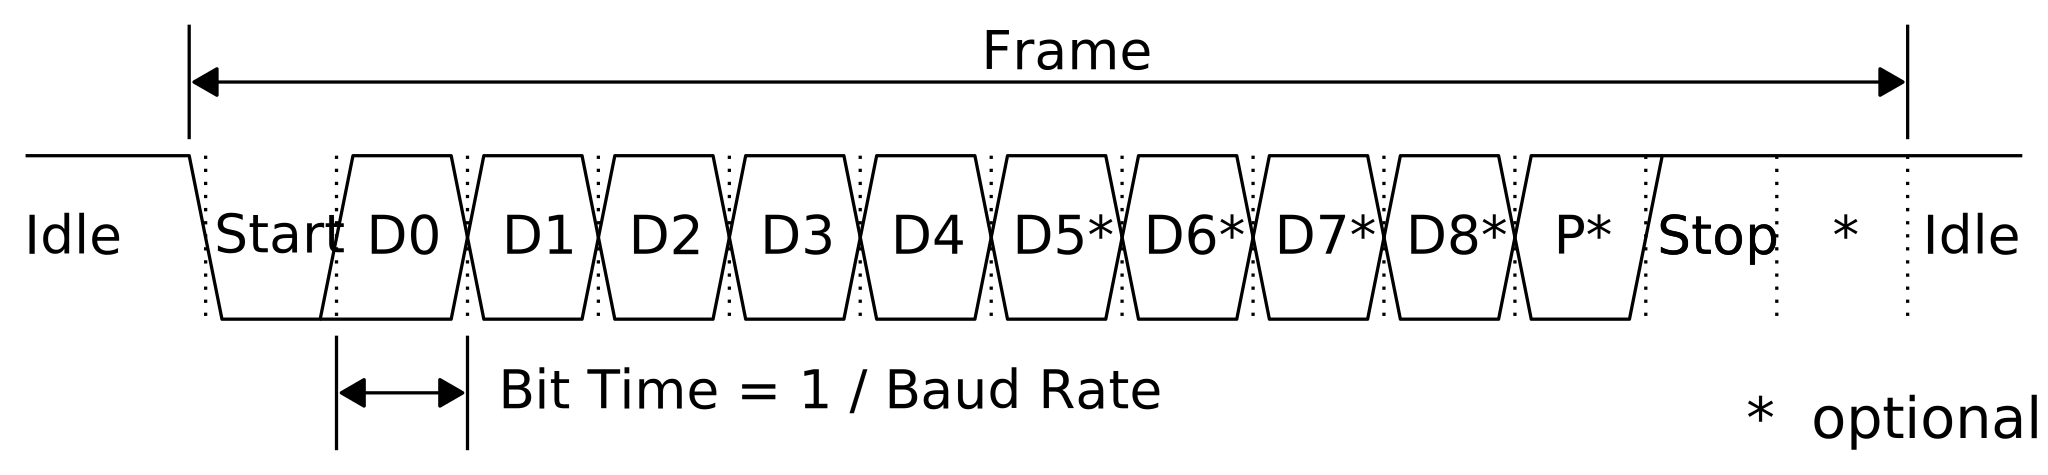
\includegraphics[width=0.8\textwidth]{serial_signals.pdf}
\end{center}
\end{frame}


\begin{frame}[shrink=5]
\frametitle{Serial Line}

Basic RS 232 specification:
\begin{itemize}
\item Designed to connect two devices only
\item Both devices are connected by a signal ground
\item 0 represented by +3 -- +15V, 1 represented by -3 -- -15V
\item Full duplex, i.e. separate signals for each transmit direction (Rx and Tx signals crossed between ends)
\item Optional handshake signals to stop transmitting when receive buffer of one or other side is getting full
\end{itemize}

Basic RS 422 specification:
\begin{itemize}
\item Differential signals, Rx+, Rx-, Tx+, Tx- -- the logical value represnetd by voltage difference (+/-) between two conductors, can be used up to 1200m distance
\item Full duplex, i.e. separate signals for each direction
\item Multiple listeners for one transmitter possible
\end{itemize}

Basic RS 485 specification:
\begin{itemize}
\item Diferential signaling same as RS 422
\item It is half-duplex - i.e. only two conductors, it is necessary disable transmitter output after sending the data and listen for othe node answer
\item Multiple devices can be interconnected, one initiator and others respond according to the address or multi-master with bus access arbitration
\end{itemize}

\end{frame}


\begin{frame}
\frametitle{UART -- Universal Asynchronous Receiver-Transmiter}

UART -- a device to receive and transmit characters/bytes over a serial line

\begin{columns}
\begin{column}{0.55\textwidth}
\begin{itemize}
  \item RX\_ST receiver status register
  \begin{itemize}
  \item bit 0 ready -- received data available
  \end{itemize}
  \item RX\_DATA received data register
  \begin{itemize}
  \item Reading from RX\_DATA removes data from UART FIFO and clears the ready flag if FIFO is empty
  \end{itemize}
  \item TX\_ST transmiter status register
  \begin{itemize}
  \item bit 0 ready -- ready to accept data to transmit
  \end{itemize}
  \item TX\_DATA data to transmit
  \begin{itemize}
  \item UART starts transmit imediatelly after write to TX\_DATA
  \end{itemize}
\end{itemize}
\end{column}
\begin{column}{0.45\textwidth}
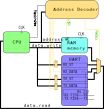
\includegraphics[width=\textwidth]{UART-en.pdf}
\end{column}
\end{columns}

\end{frame}


\begin{frame}[fragile]
\frametitle{QtRvSim Serial Port -- Terminal}

\begin{minted}[fontsize=\footnotesize]{gas}
.equ SERIAL_PORT_BASE,   0xffffc000
#base address of QtRVSim serial port

.equ SERP_RX_ST_REG,       0xffffc000  #Receiver status register
.equ SERP_RX_ST_REG_o,     0x0000      #Offset of RX_ST_REG
.equ SERP_RX_ST_REG_READY_m, 0x1 #Data byte is ready to be read
.equ SERP_RX_ST_REG_IE_m,    0x2 #Enable Rx ready interrupt

.equ SERP_RX_DATA_REG,   0xffffc004 #Received data byte in 8 LSB bits
.equ SERP_RX_DATA_REG_o,   0x0004   #Offset of RX_DATA_REG

.equ SERP_TX_ST_REG,     0xffffc008 #Transmitter status register
.equ SERP_TX_ST_REG_o,     0x0008   #Offset of TX_ST_REG
.equ SERP_TX_ST_REG_READY_m,  0x1 #Transmitter can accept next byte
.equ SERP_TX_ST_REG_IE_m,     0x2 #Enable Tx ready interrupt

.equ SERP_TX_DATA_REG,   0xffffc00c #Write word to send 8 LSB bits
.equ SERP_TX_DATA_REG_o,   0x000c   #Offset of TX_DATA_REG
\end{minted}
\end{frame}

\begin{frame}[fragile]
\frametitle{QtRvSim -- Send Character/Text String Example}

\begin{minted}[fontsize=\footnotesize]{gas}
write:
    li   a0, SERIAL_PORT_BASE # a0 set to point o UART mapping base addr.
    la   a1, text_1           # setup a1 to point to text start address
next_char:
    lb   t1, 0(a1)            # load chracter/byte from memory
    beq  t1, zero, end_char   # is this null/zero terminating character
    addi a1, a1, 1            # move pointer to next character
tx_busy:
    lw   t0, SERP_TX_ST_REG_o(a0)       # read status of transmitter
    andi t0, t0, SERP_TX_ST_REG_READY_m # mask other bits except READY
    beq  t0, zero, tx_busy    # wait/repeat if no space in UART Tx buffer
    sw   t1, SERP_TX_DATA_REG_o(a0) # tranmitter is ready - write character
    j    next_char            # process next character from the string
end_char:
    ebreak                    # stop/finish the program

    .data
text_1:
    .asciz  "Hello world.\n"  # null-character terminated text string
\end{minted}

\end{frame}

\begin{frame}[fragile]
\frametitle{QtRvSim -- Character Receive Example}

\begin{minted}[fontsize=\footnotesize]{gas}
gets: li   a0, SERIAL_PORT_BASE # a0 set to point o UART mapping base
    la   a1, text_1           # set a1 to point to start of receive buffer
    addi t2, zero, 40         # caoacity of the receive buffer
next_char:
rx_not_ready:
    lw   t0, SERP_RX_ST_REG_o(a0)       # load state of the receiver
    andi t0, t0, SERP_RX_ST_REG_READY_m # mask other bits except READY
    beq  t0, zero, rx_not_ready    # wait/repeat if no character is ready
    lw   t1, SERP_RX_DATA_REG_o(a0) # read char., it removes it from FIFO
    sb   t1, 0(a1)            # store character into buffer at a1 address
    addi t1, t1, -13          # is this new line character?
    beq  t1, zero, end_char   # if yes, branch out of the loop
    addi a1, a1, 1            # move pointer to next/free location
    addi t2, t2, -1           # subtract one from available capacity
    bne  t2, zero, next_char  # if there is space still repear receive
end_char:
    ebreak                    # stop/finish the program
    .data
text_1:
    .skip 40
\end{minted}
\end{frame}



\begin{frame}
\frametitle{QtRvSim Terminal -- Serial Port}
\begin{center}
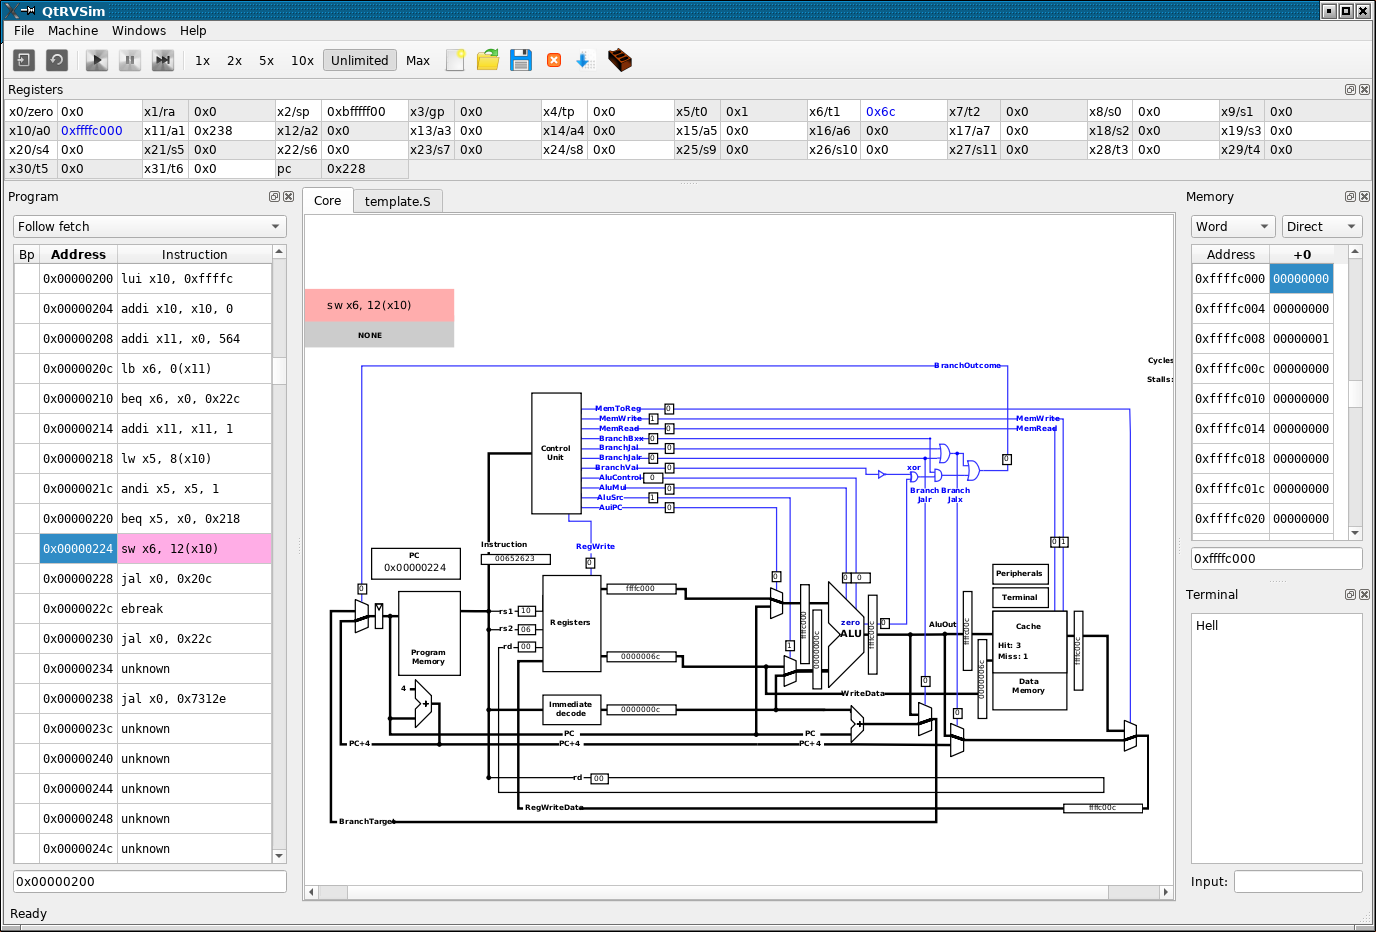
\includegraphics[width=0.8\textwidth]{fig/QtRvSim-serial-normal.png}
\end{center}
\end{frame}

\begin{frame}
\frametitle{QtRvSim Terminal -- Serial Port}
\begin{center}
Pipelined processor -- peripheral access takes place in MEM stage/phase
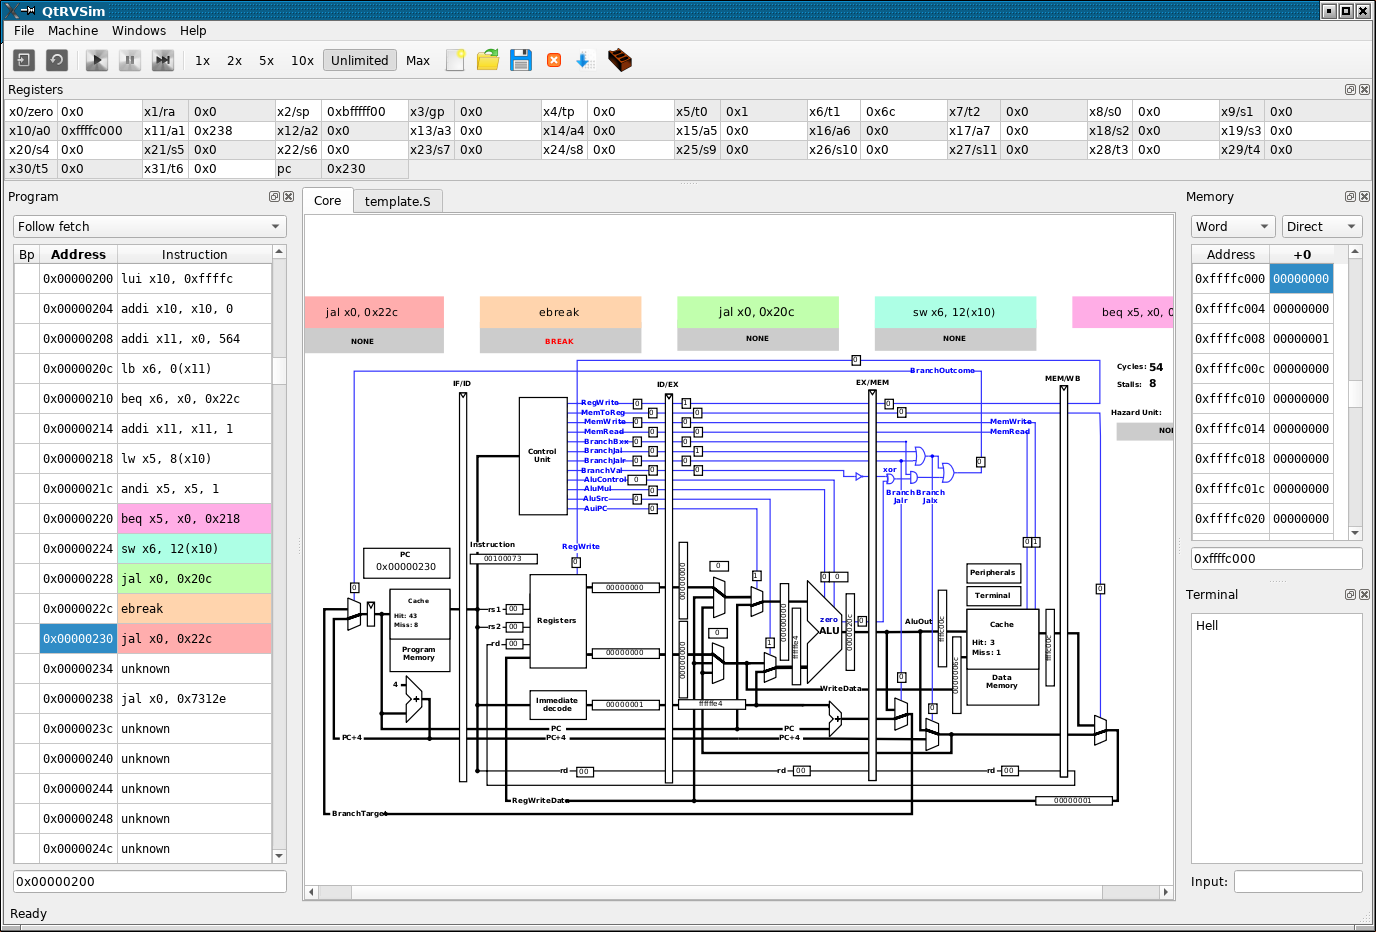
\includegraphics[width=0.8\textwidth]{fig/QtRvSim-serial-pipeline.png}
\end{center}
\end{frame}


\begin{frame}
\frametitle{Peripheral Access Summary}

\begin{itemize}
\item the above method of communication  with busy waiting is called polling
\begin{itemize}
\item the program constantly asks if something has changed, a character has been received/available or there is space in transmit queue
\item this is very inefficient, it wates CPU tie, which could be doing something useful
\end{itemize}
\item in lecture 9 we will introduce interrupts as method to notify CPU by peripherals
\begin{itemize}
\item the program can do something else, the interrupt occurs if it is enabled and the state of the peripheral changes
\item when an interrupt occurs another program/handler function starts to execute, which checks peripheal state to find which event has happened and processes it
\item information about what happened and corresponding data are passed to the program using synchronization mechanism implemented by operating system (will be discussed in detail in the OSY subject)
\end{itemize}
\end{itemize}

\end{frame}


\section{Interal Interconnection Buses}

\begin{frame}
\frametitle{A Brief History of Internal Buses in Personal Computers}

\begin{itemize}
\item ISA – an older type of passive bus, 8 or 16 bits wide, maximum transfer rate of 8 MB/s
\item PCI – a newer type of “smart” bus, 32 or 64 bits wide, burst mode, transfer rate of up to 530 MB/s, topological enumeration, Plug and Play support and programmable mapping of devices into I/O and memory address space
\item AGP – a dedicated bus designed to connect a graphics card via the northbridge to the CPU, transfer rate of 260 MB/s – 2 GB/s
\item PCI-Express (PCIe) -- a new serial implementation of the PCI bus
\end{itemize}
\end{frame}


\begin{frame}
\frametitle{Bus Topology}
Shared bus (PCI for example) -- data/address/control signals to multiple card slots
\begin{center}
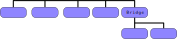
\includegraphics[width=0.8\textwidth]{shared_bus.pdf}
\end{center}

Peer-to-peer connection using a switches/hubs (e.g. PCIe, USB)
\begin{center}
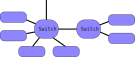
\includegraphics[width=0.65\textwidth]{switch_bus.pdf}
\end{center}
\end{frame}


\begin{frame}
\frametitle{Buses in an Older PC Computers}
\begin{center}
Old Pentium 4 architecture (1990s)
\end{center}

\begin{columns}
\begin{column}{0.5\textwidth}
The northbridge is connected directly to the CPU and the fastest peripherals -- memory and graphics card
\bigskip

The southbridge communicates with the northbridge and integrates or connects network cards, HDD, PCI slots.

\bigskip
The slowest peripherals like Floppy Disk, or serial and parallel ports (printers) are usually connected via other bridges.
\end{column}
\begin{column}{0.5\textwidth}
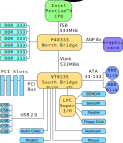
\includegraphics[width=\textwidth]{pentium4.pdf}
\end{column}
\end{columns}
\end{frame}


\begin{frame}
\frametitle{Buses in a Newer PC Computers}

\begin{center}
Modern with memory controllers on processor chip (package).
\end{center}

\begin{columns}
\begin{column}{0.4\textwidth}
The northbridge has become part of the processor.

\bigskip
The southbridge communicates directly with the processor.

\bigskip
Most peripherals are connected via PCI-Express and USB.
\end{column}
\begin{column}{0.6\textwidth}
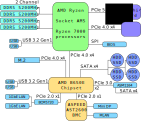
\includegraphics[width=\textwidth]{amd_am5.pdf}
\end{column}
\end{columns}
\end{frame}


\begin{frame}
\frametitle{Peripheral Component Interconnect Standard Bus -- PCI}

The all state changes and signal srobes are controlled by clock edges.

For proper operation, it needs to be synchronized as precisely as possible to the transmitted clock.

Signals marked with \# are negated because the falling edge is faster.

\begin{center}
\includegraphics[width=0.7\textwidth]{PCI_clock.pdf}
\end{center}
\end{frame}

\begin{frame}
\frametitle{PCI (Original Parallel) Bus Architecture}

\begin{columns}
\begin{column}{0.35\textwidth}
The card slot specific IDSEL signal is only for initialization, to find out what device is connected in which slot.

\medskip
AD is the 32 (64 for PCI-x) signals used for multiplexed address and data

\medskip
C/BE signals provide 4 command (transfer type) and byte enable signals

\medskip
CTRL are signals for bus transaction control (i.e. FRAME)
\end{column}
\begin{column}{0.6\textwidth}
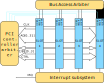
\includegraphics[width=\textwidth]{PCI_arch-en.pdf}
\end{column}
\end{columns}

\end{frame}


\begin{frame}
\frametitle{PCI Data Transfers -- Write Transaction}

\begin{itemize}
\item The initiator begins the transfer by request for bus control to arbiter
\begin{itemize}
\item If multiple devices request the bus at the same time, the arbiter must queue their requests and allow only one transfer at a time
\end{itemize}
\item The initiator begins the transmission by setting the address of the target peripheral register on the AD bus and asserting (active low) the FRAME signal; the first clock rising edge address is strobed, next is data, the last data transfer is denoted by the deassertion of FRAME
\end{itemize}

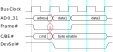
\includegraphics[width=0.8\textwidth]{PCI_write1.pdf}

\end{frame}

\begin{frame}
\frametitle{PCI Data Transfers -- Write Transaction -- Data}

\begin{itemize}
\item A peripheral that recognizes its address asserts DevSel
\item If the target peripheral (Target) is ready to receive data, it asserts TRDY.
\item If the initiator is ready to send data, it asserts IRDY.
\end{itemize}

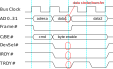
\includegraphics[width=0.8\textwidth]{PCI_write2-en.pdf}

\end{frame}


\begin{frame}
\frametitle{PCI Data Transfers -- Write Transaction -- Wait}

\begin{itemize}
\item If the target peripheral is not ready, it deasserts TRDY
\item If the initiator is not ready to put data on the bus, it deasserts IRDY
\item If TRDY or IRDY is not asserted, then the data transfer is suspended -- wait for state at next clock edge
\end{itemize}

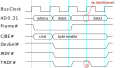
\includegraphics[width=0.8\textwidth]{PCI_write3-en.pdf}

\end{frame}


\begin{frame}
\frametitle{PCI Data Transfers -- Write Transaction -- the Last Data}

\begin{itemize}
\item Deasserts the FRAME signal to inform that the last data will be sent
\item In the shown case, the data transfer was suspended, so the transfer of the last data is postponed to the next clock cycle.
\end{itemize}

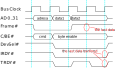
\includegraphics[width=0.8\textwidth]{PCI_write4-en.pdf}

\end{frame}

\begin{frame}
\frametitle{PCI Data Transfers -- Write Transaction -- Release Bus}

\begin{itemize}
\item After the transfer is completed (the last data sent and accepted), the IRDY, TRDY and DEVSEL signals are deasserted and the bus is released for the next transfer.
\end{itemize}

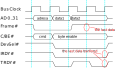
\includegraphics[width=0.8\textwidth]{PCI_write4-en.pdf}

\end{frame}


\begin{frame}
\frametitle{PCI Data Transfers -- Read Transaction}

\begin{itemize}
\item The initiator requests data from the target peripheral.
\item Data transfer is similar, but cannot start on the next clock cycle because the initiator must disconnect from the AD bus and the target device must connect its output buffer to the bus.
\end{itemize}

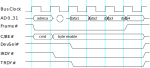
\includegraphics[width=0.8\textwidth]{PCI_read1.pdf}

\end{frame}


\begin{frame}
\frametitle{Classical Parallel PCI Bus -- Summary}

Disadvantages of the PCI bus:
\begin{itemize}
\item Half-duplex data cannot be sent in both directions at the same time, data transferred in only one direction at time
\item Multiple devices on the shared bus -- slow peripherals slow down fast peripherals, increases the latency of all other peripherals
\item PCI bus only allows clocks with 33\,MHz, or 66\,MHz
\begin{itemize}
\item This corresponds to 132\,MB/s or 264\,MB/s for the 32-bit variant
\item This corresponds to 264\,MB/s or 528\,MB/s for the 64-bit variant
\end{itemize}
\item PCI eXtended (PCI-X) bus allows clocks up to 133 MHz and later a maximum of 533 MHz
\begin{itemize}
\item This corresponds to transfer speeds of 532MB/s to a maximum of 4266 MB/s for the 64-bit variant variant, very hard to route on PCB
\item PCI-X version 2.0 with speeds above 133MHz were not very widespread
\end{itemize}
\item The connector for the 32-bit version has 62 pins -- i.e. 124 signals, for the 64-bit version it is even 188 signals
\end{itemize}

\end{frame}


\begin{frame}
\frametitle{PCI Expres -- PCIe}

The main disadvantage of parallel busses is the required precise mutual matching of the signals delays and routing:
\begin{itemize}
\item Even small inaccuracies in the length of the conductors and the quality of the connections lead to different propagation speed/delay of the electrical signal
\item No problem for low frequencies but even small mutual and or clocks timing shift prevents consistent data strobing over multiple wires for high ones.
\item It is demostrated in animation at https://cw.fel.cvut.cz/wiki/courses/b35apo/en/lectures/07/start
\end{itemize}
\smallskip

\begin{columns}[T]
\begin{column}{0.32\textwidth}
frequency $f$
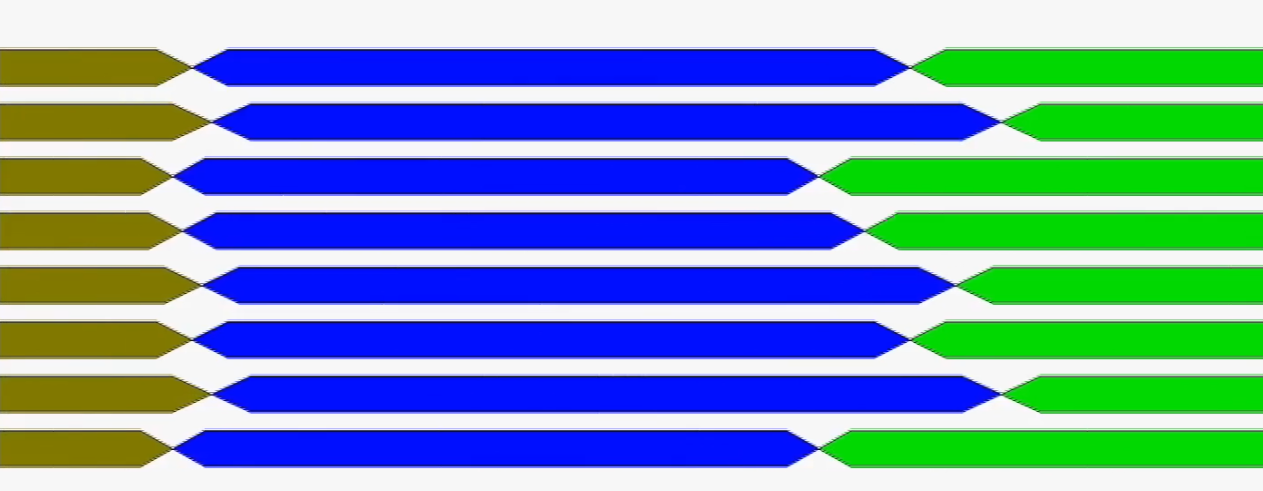
\includegraphics[width=\textwidth]{fig/freq1.png}
transfer without problems
\end{column}
\begin{column}{0.32\textwidth}
frequency $2\cdot f$
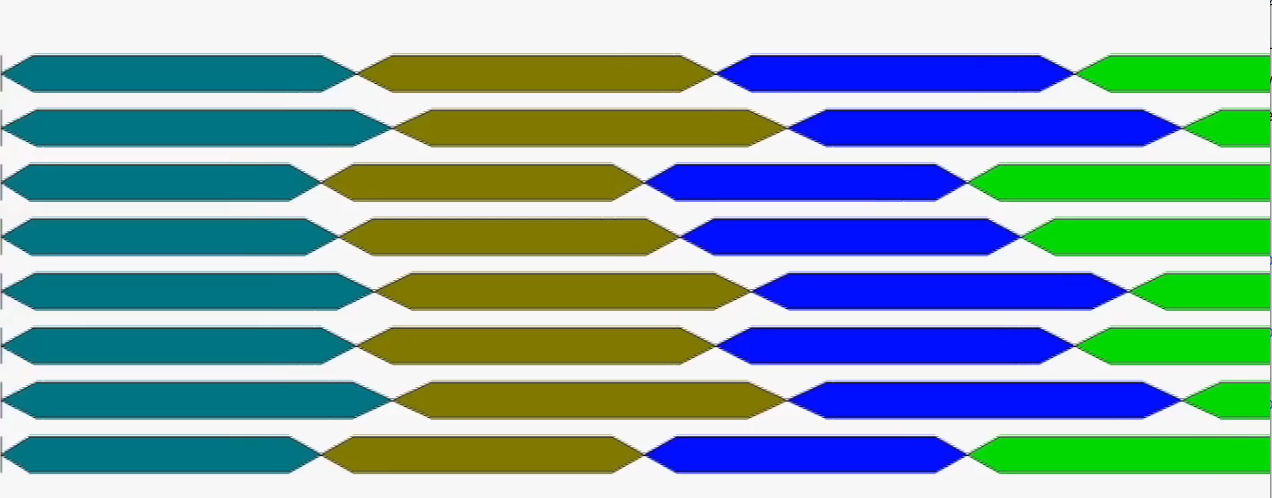
\includegraphics[width=\textwidth]{fig/freq2.png}
transfer at reliability limit
\end{column}
\begin{column}{0.32\textwidth}
frequency $4\cdot f$
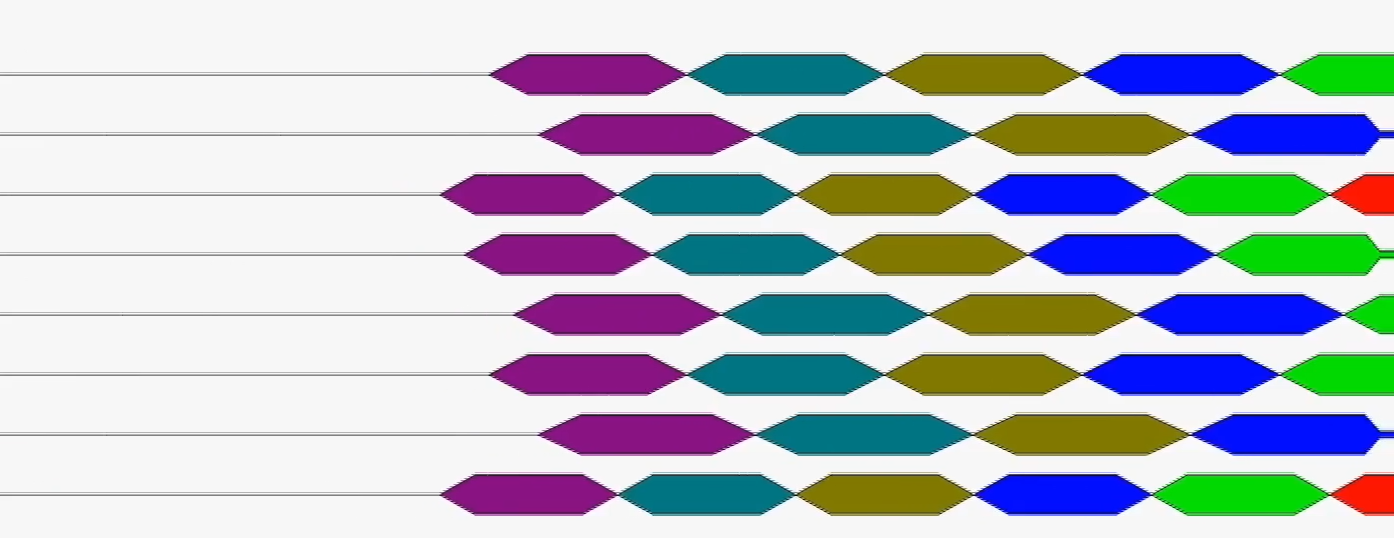
\includegraphics[width=\textwidth]{fig/freq4.png}
no instant to strobe parallel data by receiver
\end{column}
\end{columns}

\end{frame}


\begin{frame}
\frametitle{PCI-Express (PCIe) -- Upgrades to Parallel PCI}

\begin{itemize}
\item PCIe is peer-to-peer -- signals are only routed between two devices.
\item PCIe is full-duplex -- data can be transferred in both directions at the same time.
\item For one-way transmission, a serial method with differential signal pair (per lane) is used, rejects common mode voltage shifts and noises
\begin{itemize}
\item This method of transmission is less susceptible to interference than a single ended wire to ground.
\end{itemize}
\item PCIe can contain multiple links, but the transmission between the links is not synchronized at the bit level.
\item In the simplest version, PCIe connectors have only 18 pins, 36 signals, of which 18 are ground and power.
\end{itemize}

\end{frame}

\begin{frame}
\frametitle{PCIe Serial Transmission}

\begin{itemize}
\item PCIe can use different speeds for transmission
\item It is necessary that the receiving side can detect the transmission speed.
\item The problem is that if a byte contains only 0s or only 1s, the signal does not change.
\item The solution is to encode a byte (8 bits) into 10 bits so that the total number of 0s and 1s transmitted is the same.
\end{itemize}

Quiz: How many different 10-bit numbers are there that have five 0s and five 1s?

\begin{itemize}
\item[A] $2^5 \cdot 2^5 = 64$
\item[B] $5! \cdot 5! = 14400$
\item[C] ${10 \choose 5} = 252$
\item[D] $5! + 5! = 240$
\end{itemize}
\end{frame}


\begin{frame}
\frametitle{PCIe 8b/10b Encoding}

\begin{itemize}
\item 8 bits, or 256 different values, are encoded into a 10-bit number that has at least four 0s and at least four 1s
\begin{itemize}
\item This extends to ${10 \choose 5} + 2\cdot {10 \choose 6}= 672$ of such 10-bit numbers
\item We choose those codes where are more 1 $\rightarrow$ 0 and 0 $\rightarrow$ 1 transitions.
\end{itemize}
\item For codes where cound of 0s and 1s differs (by one only), there is freedom whether code with more 1s or matching complement with more 0s is chosen
\end{itemize}

\bigskip
table to code 3b by 4b\phantom{xxxxx}{
\scriptsize
\begin{tabular}{|c|c|c|c|}\hline
\multicolumn{2}{|c|}{Input} & RD = −1 &	RD = +1 \\\hline
Code & HGF & \multicolumn{2}{c|}{f g h j} \\\hline
D.x.0 &000 &1011 & 0100\\\hline
D.x.1 &001 &\multicolumn{2}{c|}{1001}\\\hline
D.x.2 &010 &\multicolumn{2}{c|}{0101}\\\hline
D.x.A3 &011 &\multicolumn{2}{c|}{1100}\\
D.x.B3 &    &\multicolumn{2}{c|}{0011}\\\hline
D.x.4 &100 &1101 &0010\\\hline
D.x.5 &101 &\multicolumn{2}{c|}{1010}\\\hline
D.x.6 &110 &\multicolumn{2}{c|}{0110}\\\hline
D.x.P7 & 111 &1110 & 0001\\
D.x.A7 & &  0111 & 1000\\\hline
\end{tabular}
}
\end{frame}


\begin{frame}
\frametitle{PCIe Versions 1.x and 2.x}

Ver 1.x
\begin{itemize}
\item The transfer rate is 2.5\,GT/s (transfers per second, number of symbols per second on one lane)
\item 10 transfers are required for one byte of 8 bits
\item The maximum bandwidth (transfer capacity) is therefore 250\,MB/s = $(2500 \cdot \frac{8}{10})$ Mb/s = $(2500 \cdot \frac{1}{10})$\,MB/s, practical with headers 200\,MB/s per lane
\item PCIe allows up to 16 independent links (lanes) for one peripheral connection, data bytes transferred independently in parallel
\begin{itemize}
\item The maximum bandwidth is $(16 \cdot 250)$\,MB/s = $4$\,GB/s
\end{itemize}
\end{itemize}

Ver 2.x
\begin{itemize}
\item The transfer rate is 5\,GT/s (transfers per second)
\item 10 transfers are required for one byte of 8 bits
\item The maximum bandwidth of one line (x1) is 500\,MB/s
\item The maximum bandwidth for 16 links (x16) is $(16 \cdot 500)$ MB/s = $8$ GB/s
\end{itemize}
\end{frame}


\begin{frame}
\frametitle{PCIe Vresion. 3.x, 4.x and 5.x}

8b/10b encoding is unnecessarily inefficient, 128b/130b encoding with similar parameters was chosen.
\begin{itemize}
\item Ver 3.x
\begin{itemize}
\item The transfer rate is 8\,GT/s (transfers per second)
\item The maximum transfer capacity is therefore almost 985\,MB/s = $(8000 \cdot \frac{128}{130})$\,Mb/s = $(8000 \cdot \frac{16}{130})$\,MB/s
\item The maximum bandwidth for x16 is $(16 \cdot 985)$\,MB/s = $15.75$ GB/s
\end{itemize}
\item Ver 4.x
\begin{itemize}
\item The transfer rate is 16\,GT/s (transfers per second)
\item The maximum bandwidth is therefore almost 1.97\,GB/s = $(16000 \cdot \frac{16}{130})$ MB/s
\item The maximum bandwidth for x16 is $(16 \cdot 1.97)$\,GB/s = $31.5$\,GB/s
\end{itemize}
\item Ver 5.x
\begin{itemize}
\item The transfer rate is 32\,GT/s (transfers per second)
\item The maximum bandwidth is therefore almost 3.94\,GB/s = $(32000 \cdot \frac{16}{130})$\,MB/s
\item The maximum bandwidth for x16 is $(16 \cdot 3.94)$\,GB/s = $63$\,GB/s
\end{itemize}
\end{itemize}

\end{frame}

\begin{frame}
\frametitle{PCIe Topology}

Communication over the PCIe bus is similar to communication over a swiched network (i.e. Ethernet).
\begin{itemize}
\item Communication takes place in packets
\begin{itemize}
\item ATTENTION -- packet overhead is not included in the maximum transmission capacity.
\item Each packet has a synchronization header, address, data, crc -- similar to the Ethernet protocol.
\end{itemize}
\item The use of switches is similar to that in a network
\begin{itemize}
\item Switches allow direct communication only between two devices
\item Switches can prioritize packets -- advantageous for reducing latency (using packets, on the other hand, increases latency)
\item Switches can be used to ensure automatic detection and configuration of connected devices on a similar principle to that of the PCI bus
\end{itemize}
\end{itemize}

\end{frame}


\begin{frame}
\frametitle{The Reality of Serial Bus Signals}

High-speed communication presents many different problems.

Signal Appearance over Distance

\begin{center}
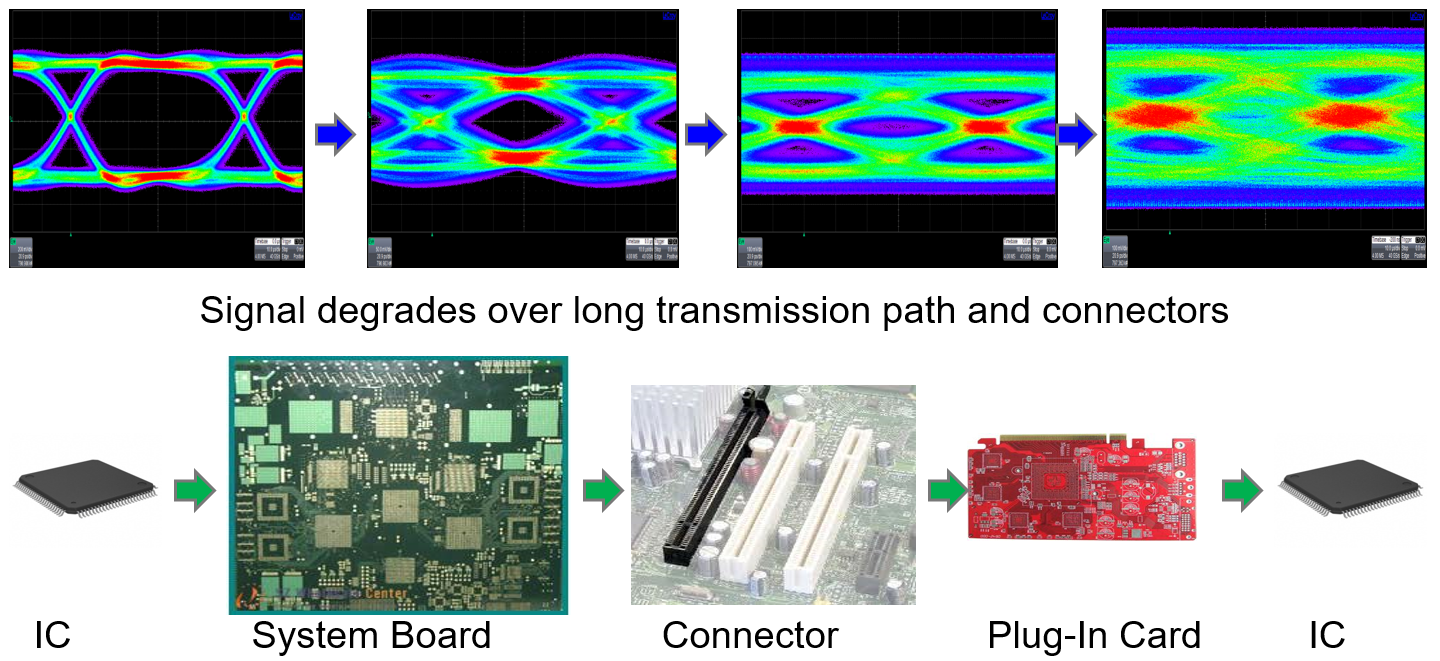
\includegraphics[width=0.8\textwidth]{fig/signals.png}
\end{center}

\end{frame}


\begin{frame}
\frametitle{Hard Drives and SSD Storage}

\begin{itemize}
\item A similar development to the change from PCI to PCIe can be observed in drives.
\item PATA or Parallel ATA is a parallel drive connection since 1984 for the first IBM PC/AT
\begin{itemize}
\item The name ATA actually stands for AT Attachment, AT is an abbreviation for Advance Technology.
\item Also referred to as IDE, later Extended IDE (EIDE) Utra ATA (UATA)
\item PATA is a 16-bit parallel data transfer between the CPU and the drive
\item In its fastest version, it could transfer up to 133 MB/s
\end{itemize}
\item SATA is a serial version of disk communication.
\begin{itemize}
\item In the minimum version, it only needs 7 wires, A+, A-, B+, B- and 3x ground.
\begin{itemize}
\item SATA 1.0: 150MB/s (PATA:130MB/s)
\item SATA 2.0: 300 MB/s
\item SATA 3.0: 600 MB/s
\item SATA 3.2: about 2 GB/s
\end{itemize}
\end{itemize}
\end{itemize}
\end{frame}


\end{document}

